
\documentclass[preprint]{elsarticle}
\usepackage{amsmath,amssymb,graphicx,booktabs}
\usepackage{float}     % nel preambolo del SI
\graphicspath{{../}{./}}

% numerazione S1, S2, ... per figure, tabelle ed equazioni
\renewcommand{\thefigure}{S\arabic{figure}}
\renewcommand{\thetable}{S\arabic{table}}
\renewcommand{\theequation}{S\arabic{equation}}
\renewcommand{\thesection}{S\arabic{section}}   % anche le sezioni

\begin{document}
\begin{frontmatter}
\title{Supplementary Material for\\
  ``Semantic burstiness across principal directions of textual
  variation''}
\author[unibo]{Mirko Degli Esposti}
\author[ou]{Marcelo A. Montemurro}
\affiliation[unibo]{organization={Department of Physics and Astronomy,
  University of Bologna}, city={Bologna}, country={Italy}}
\affiliation[ou]{organization={School of Mathematics and Statistics,
  The Open University}, city={Milton Keynes}, country={United Kingdom}}
\end{frontmatter}

\section{Inter-event-time distributions for the remaining representative texts}
\label{app:pertext}

Inter-event-time distributions for the three representative texts
other than \emph{War and Peace}, whose corresponding figure appears in
the main text. Equivalent figures for every text of the corpus, at any
threshold quantile, can be regenerated with \texttt{scripts/run\_text.py}
in the code repository.


\begin{figure}[H]
  \centering
  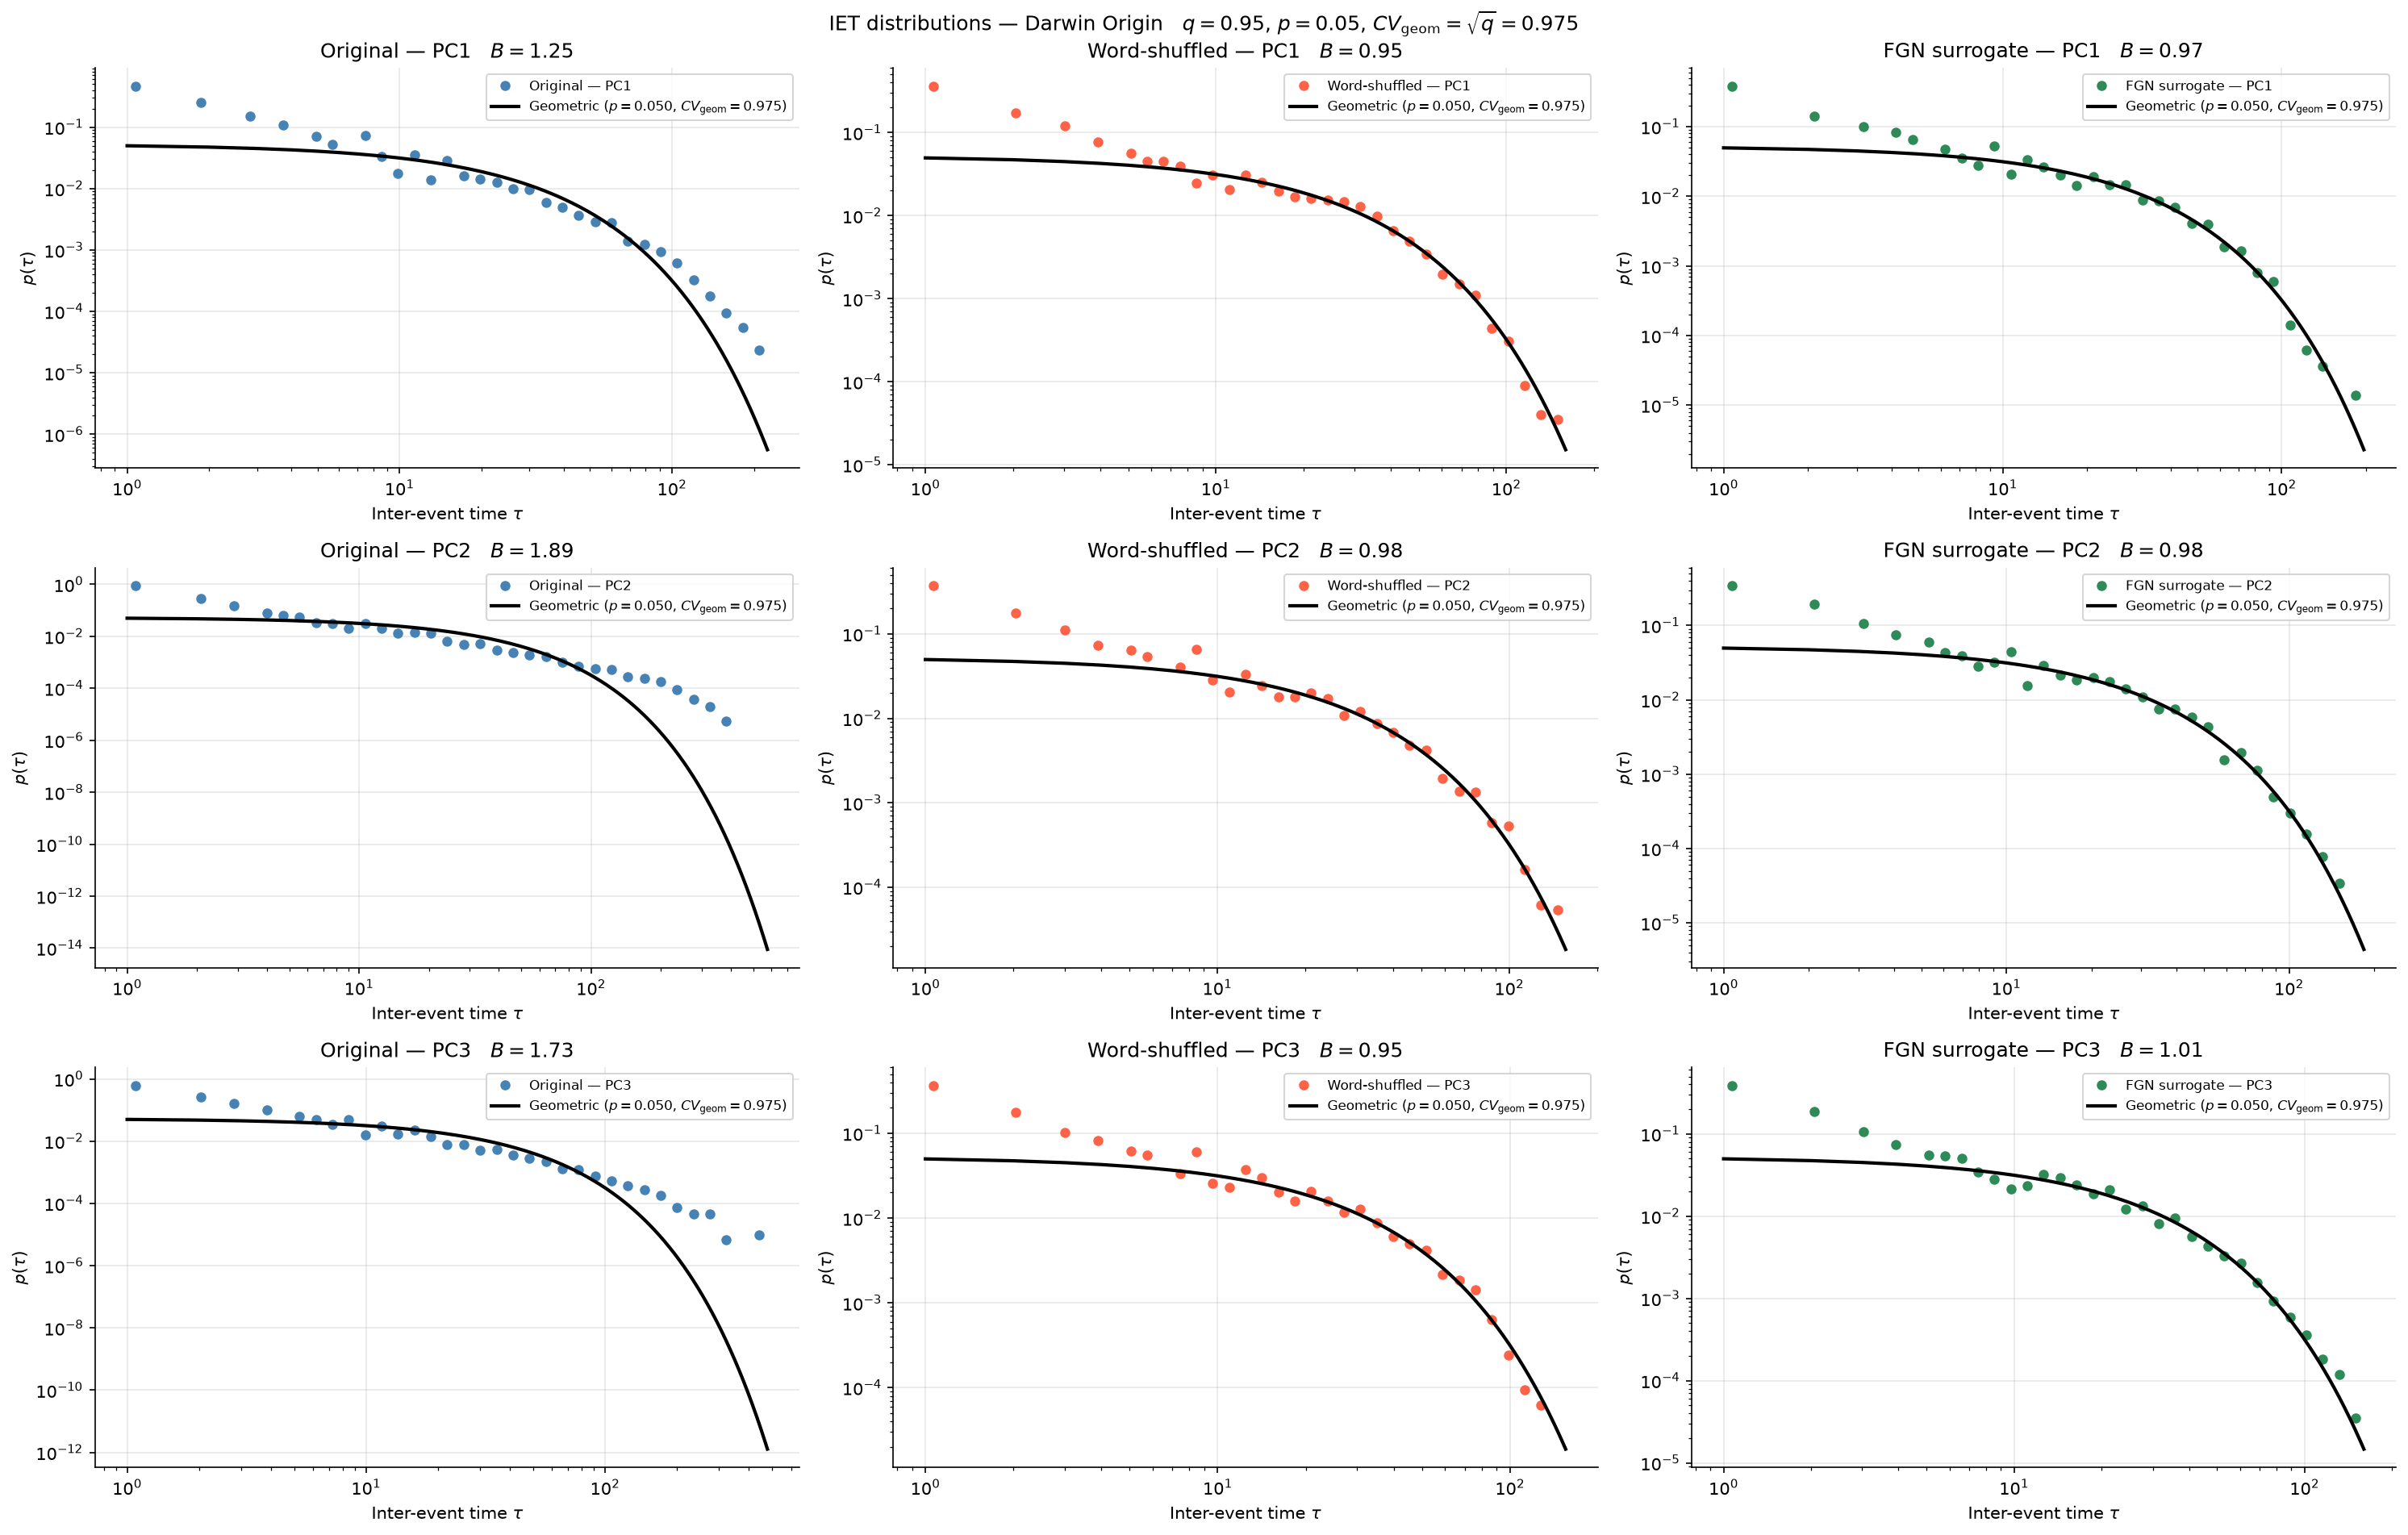
\includegraphics[width=\textwidth]{figures/darwin_origin/darwin_origin_03_iet_comparison.png}
  \caption{Inter-event time distributions for PC1, PC2, PC3 of
  \emph{On the Origin of Species} ($q=0.95$).
  Same conventions as the corresponding figure in the main text.}
  \label{fig:darwin_iet}
\end{figure}

\begin{figure}[H]
  \centering
  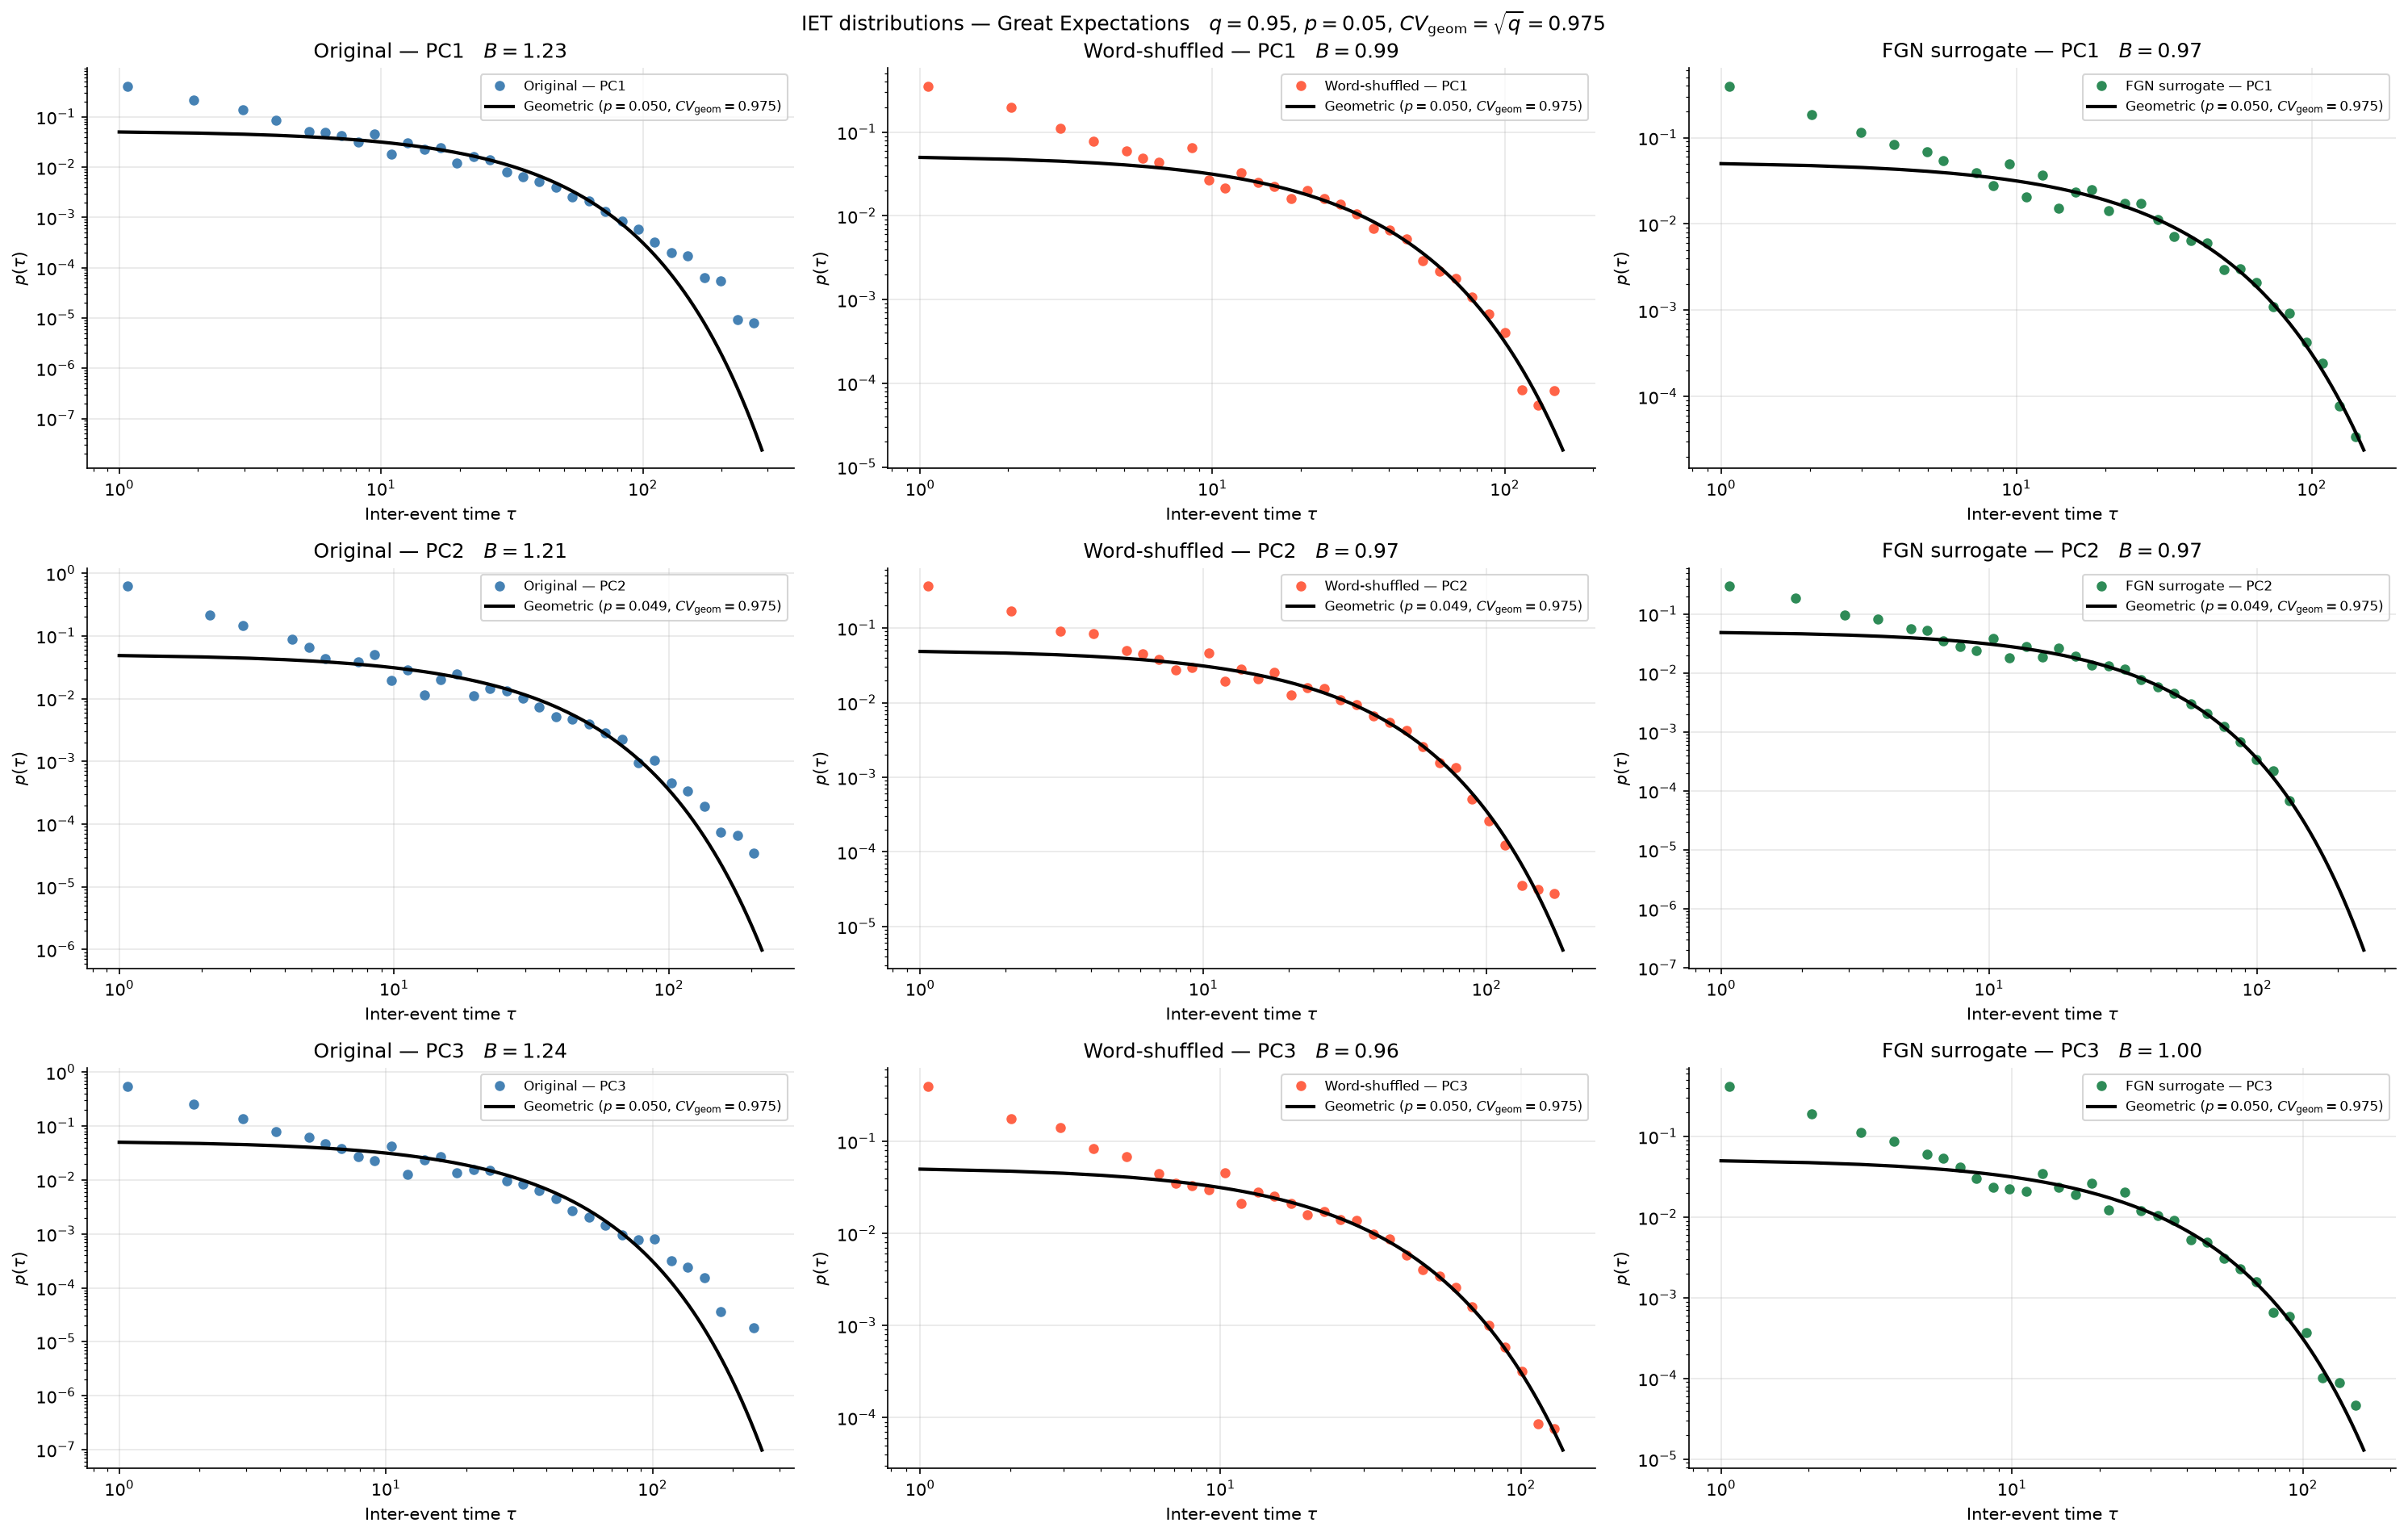
\includegraphics[width=\textwidth]{figures/great_expectations_cut_clean/great_expectations_cut_clean_03_iet_comparison.png}
  \caption{Inter-event time distributions for PC1, PC2, PC3
  of \emph{Great Expectations} ($q=0.95$).
  Same conventions as the corresponding figure in the main text.}
  \label{fig:greatexp_iet}
\end{figure}

\begin{figure}[H]
  \centering
  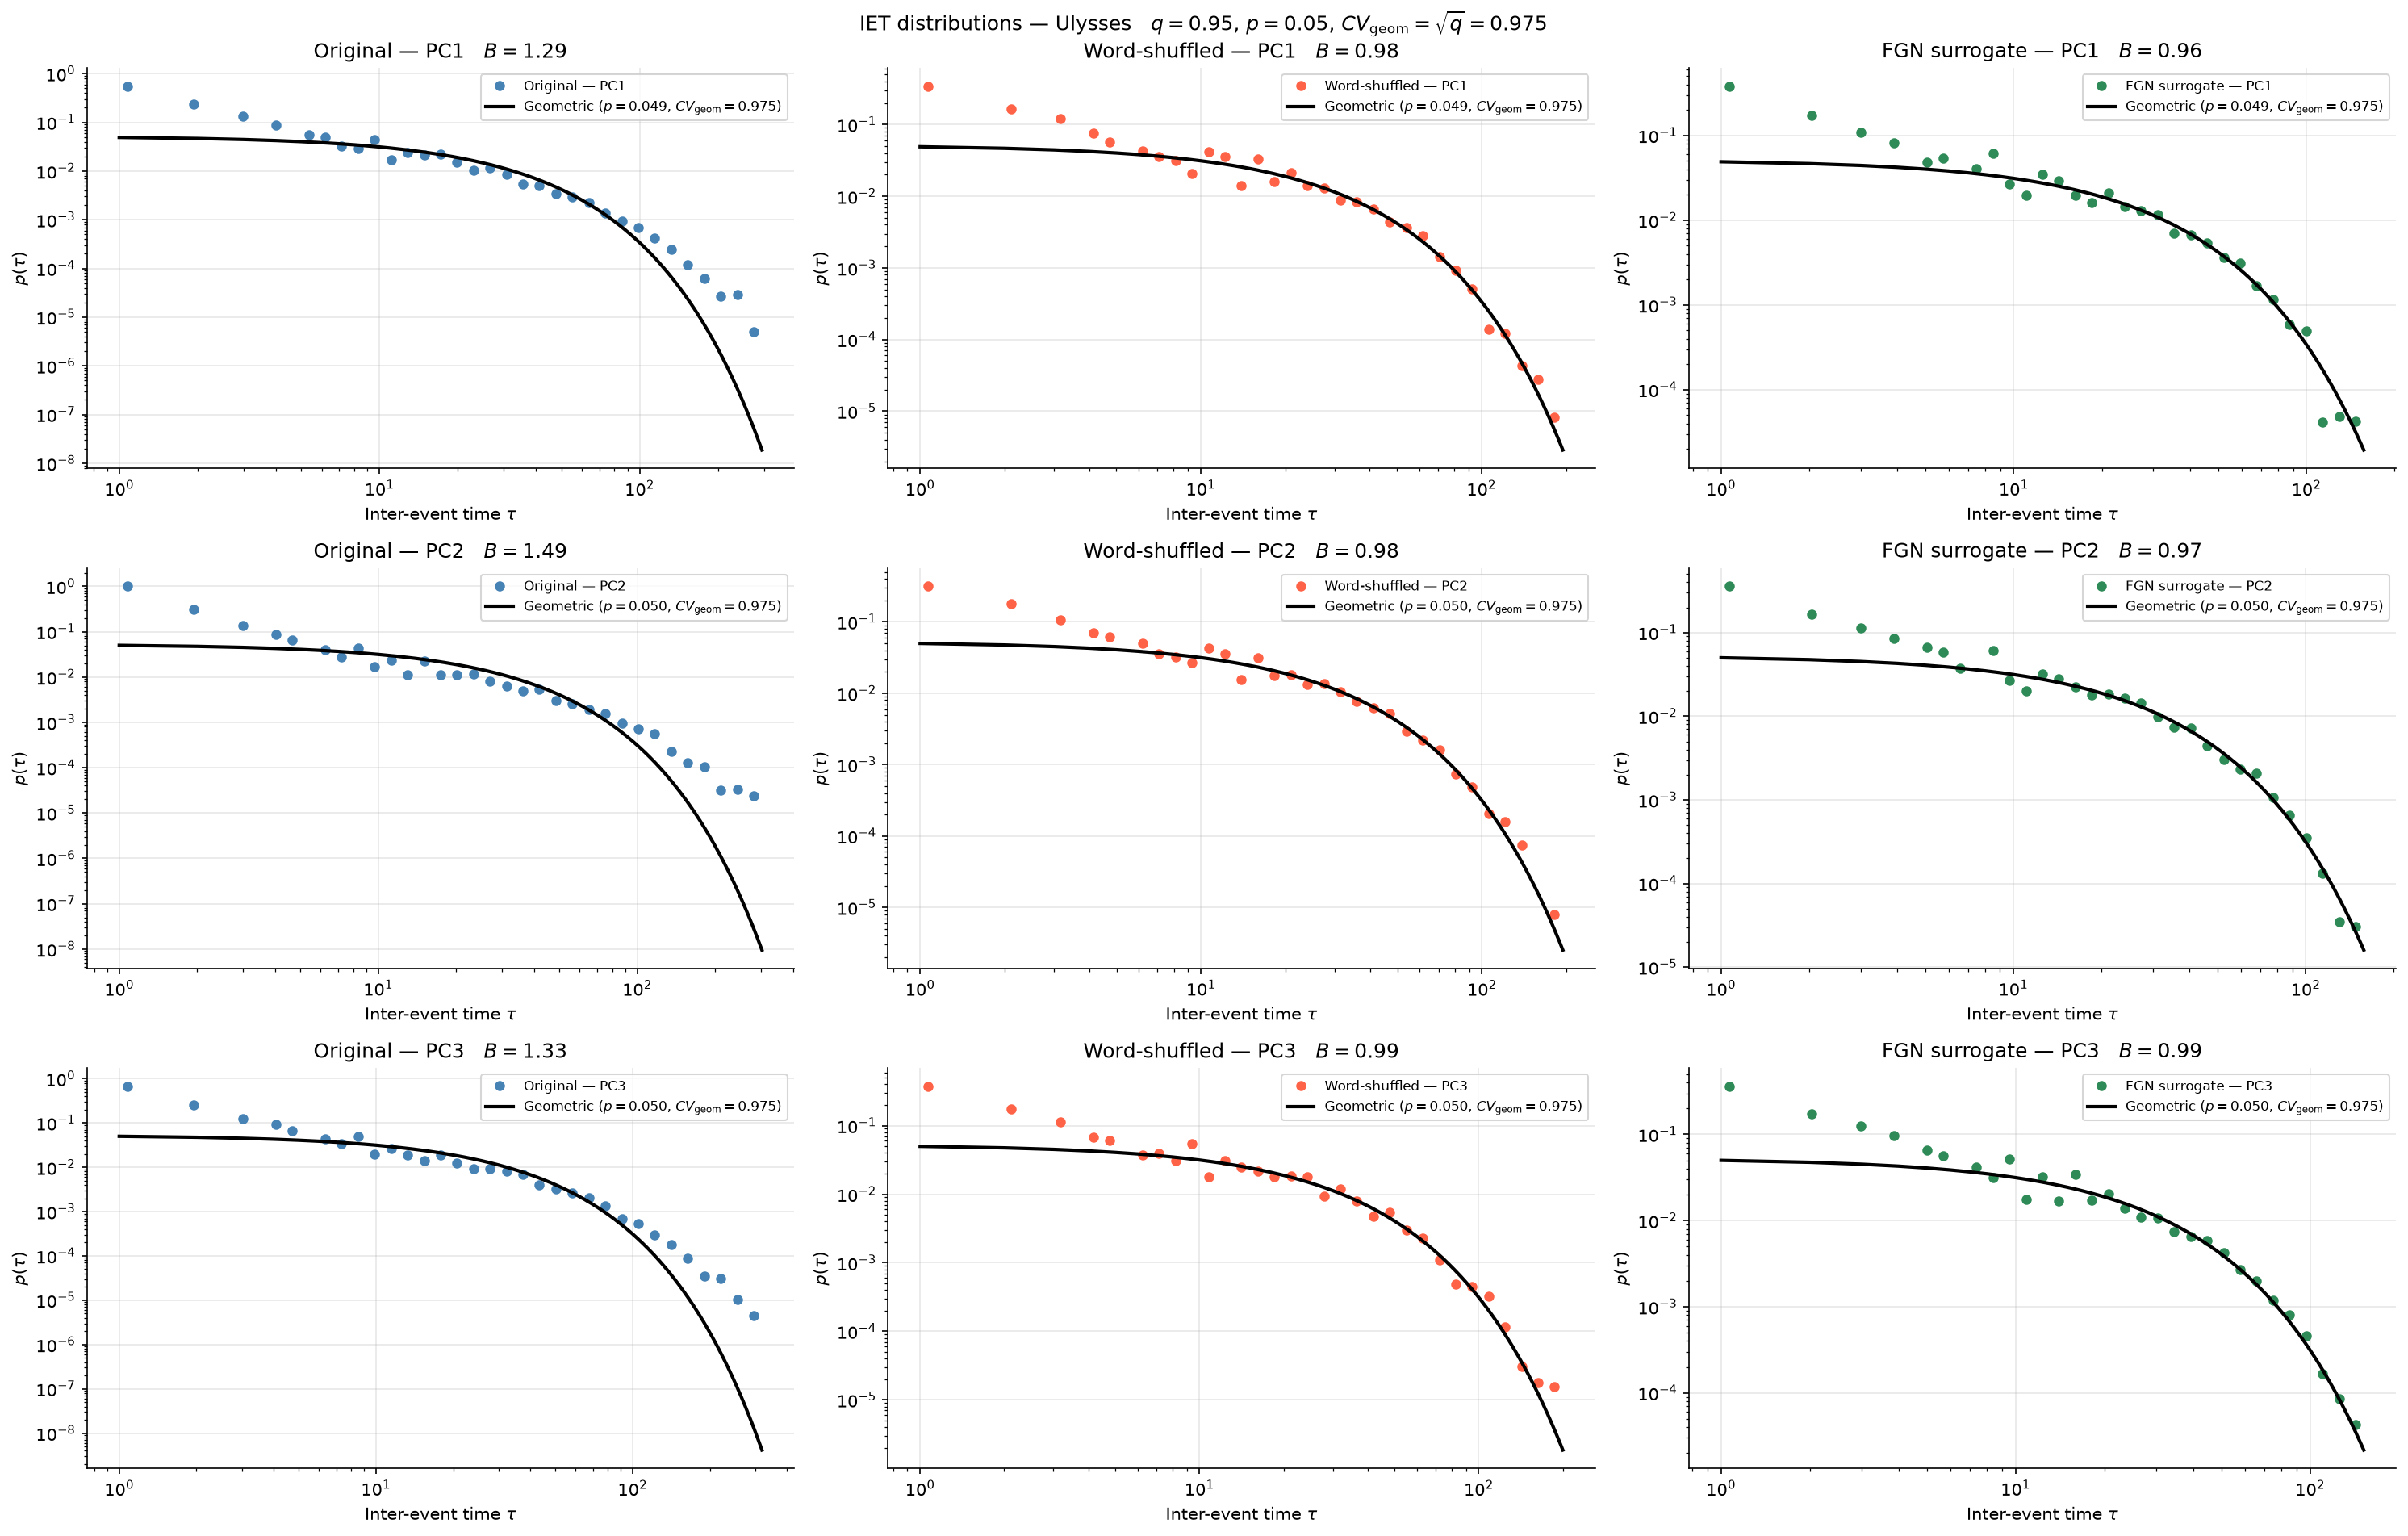
\includegraphics[width=\textwidth]{figures/eng_ulysses/eng_ulysses_03_iet_comparison.png}
  \caption{Inter-event time distributions for PC1, PC2, PC3
  of \emph{Ulysses} ($q=0.95$).
 Same conventions as the corresponding figure in the main text.}
  \label{fig:ulysses_iet}
\end{figure}


\clearpage
\section{Additional robustness figures}
% corpus_robustness, corpus_diffs, acf_corpus_frac, acf_corpus_rho1, acf_mean

\begin{figure}[H]
  \centering
  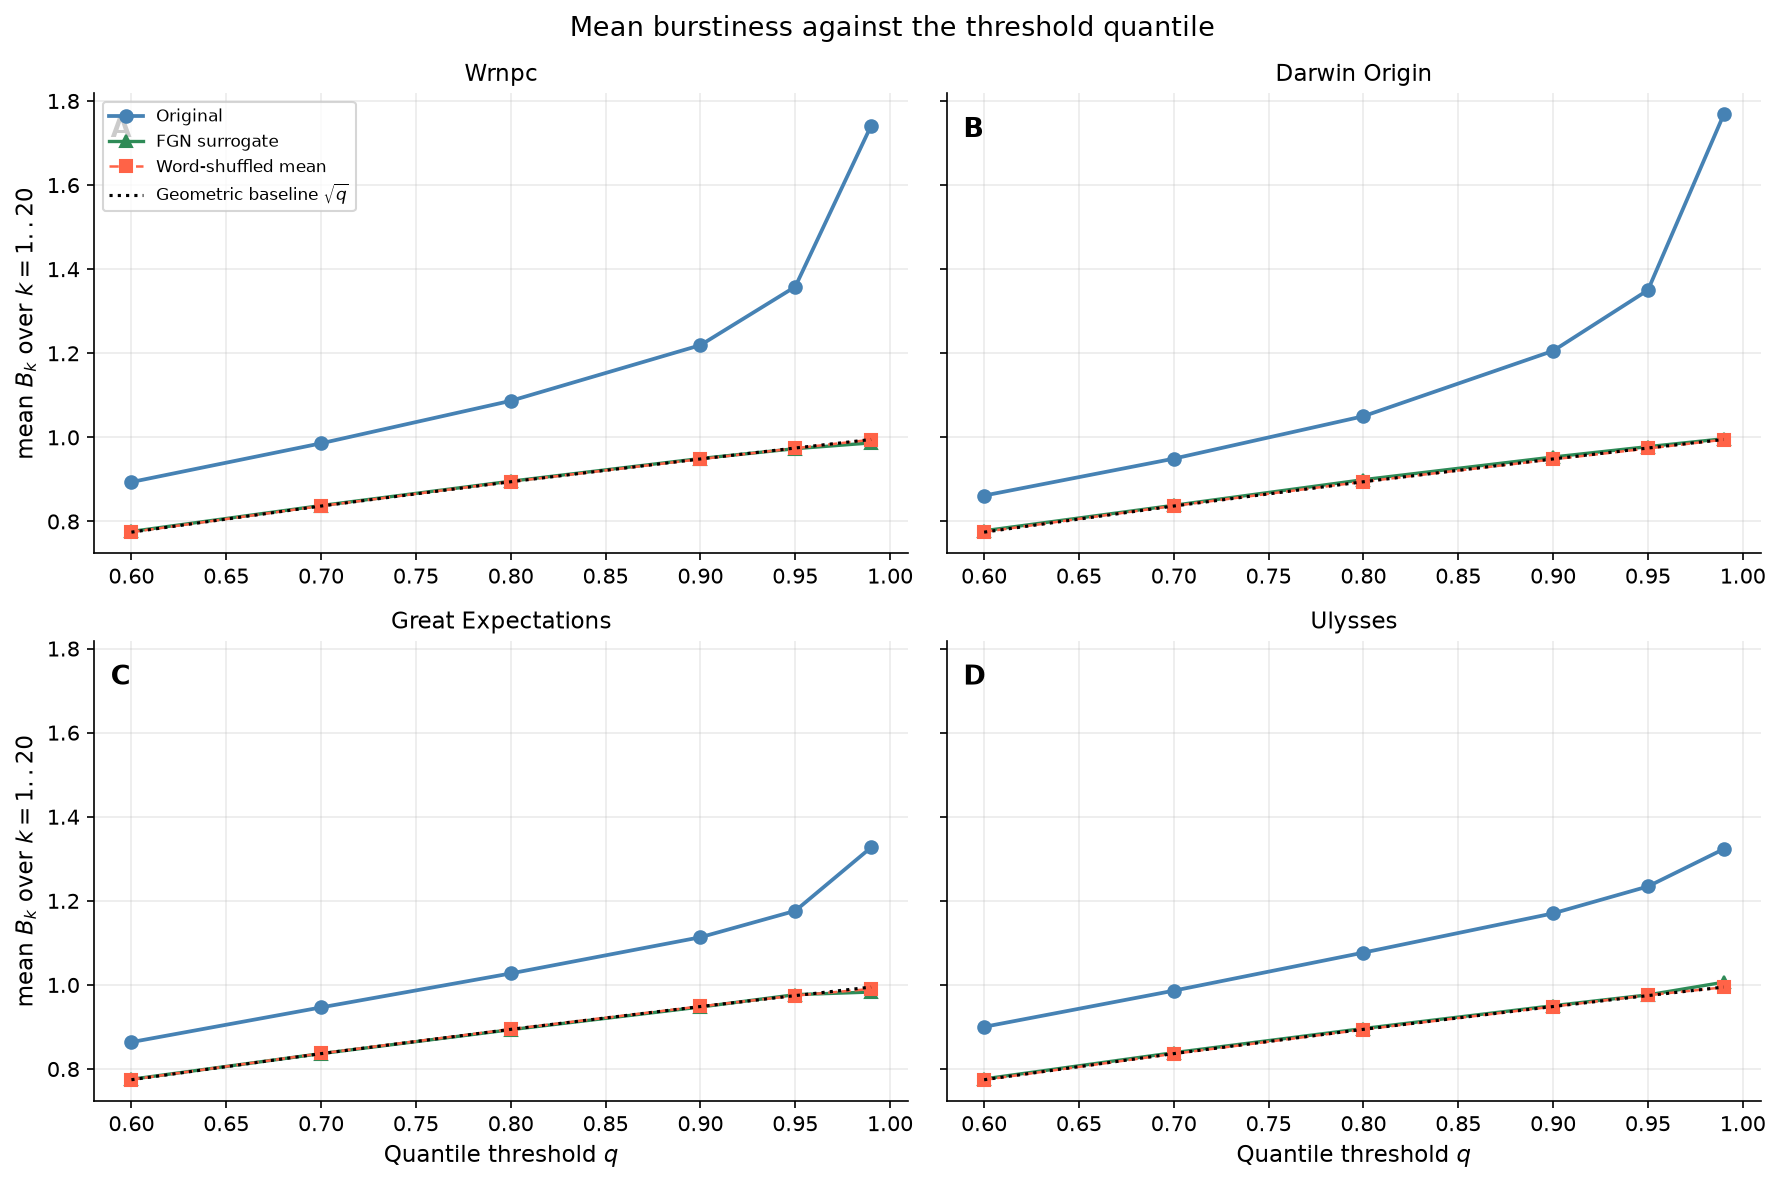
\includegraphics[width=\textwidth]{figures/panel_quantile_sweep.png}
  \caption{Mean burstiness over $k=1,\ldots,20$ as a function of the
  threshold quantile $q$, for the four representative texts:
  \textbf{A} \emph{War and Peace}, \textbf{B} \emph{On the Origin of
  Species}, \textbf{C} \emph{Great Expectations}, \textbf{D}
  \emph{Ulysses}. The original stays above both controls and above the
  geometric baseline $\sqrt{q}$ throughout $q \in [0.60, 0.99]$, and the
  full ordering $B_k^{\rm orig} > B_k^{\rm FGN}$ and
  $B_k^{\rm orig} > B_k^{\rm surr}$ holds for all 20 components at every
  displayed $q$ in each text. Absolute burstiness grows towards more
  extreme thresholds, as rare visits to the upper tail accentuate
  episode-to-episode clustering.}
  \label{fig:sweep_panel}
\end{figure}

\begin{figure}[H]
  \centering
  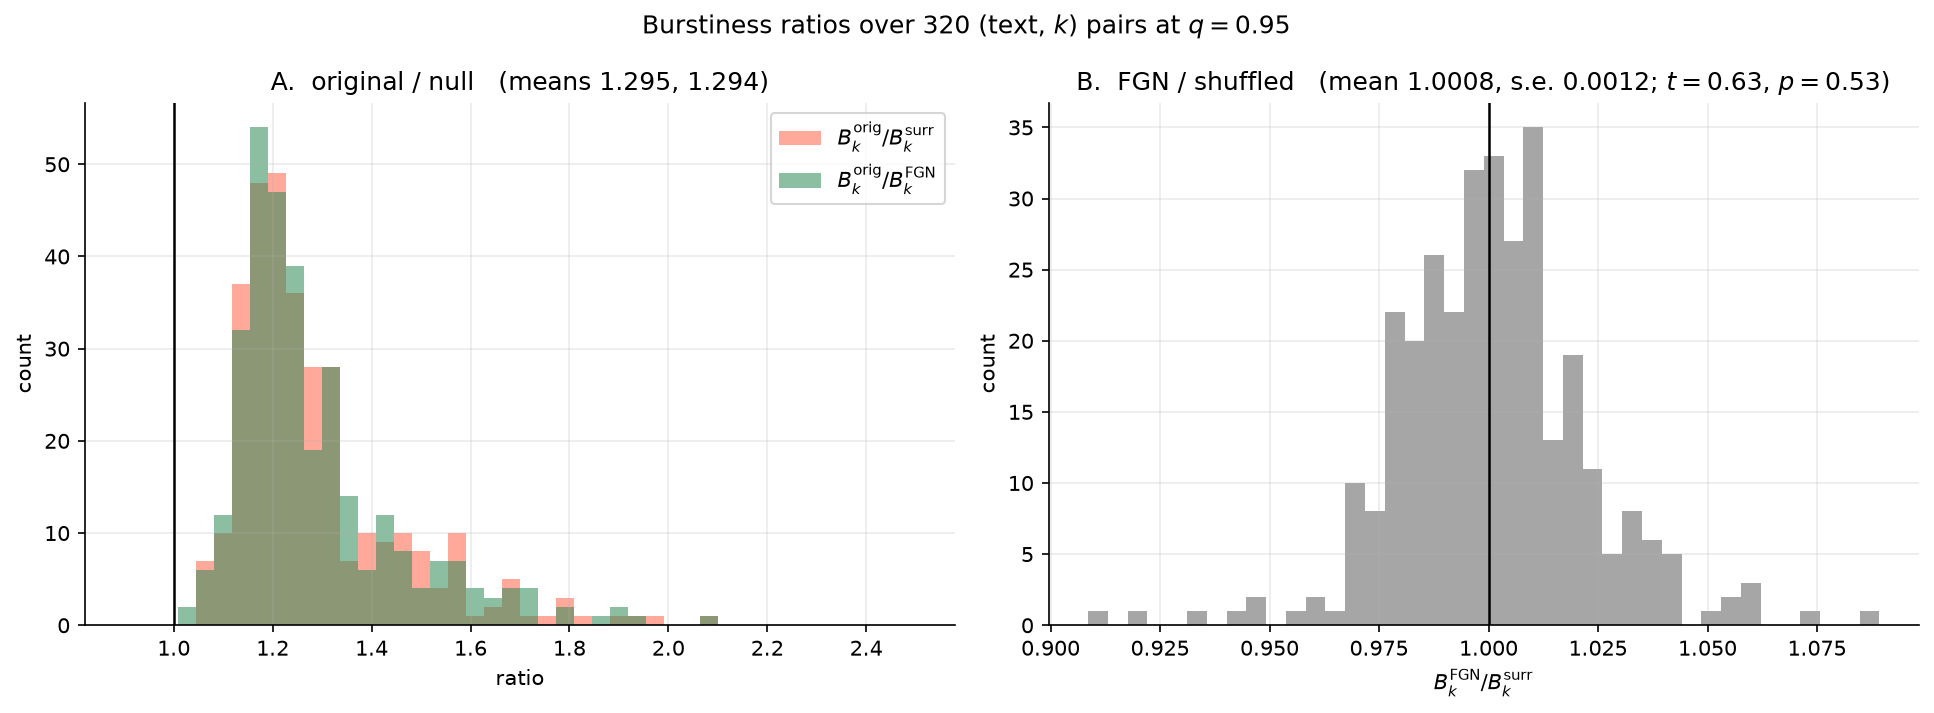
\includegraphics[width=\textwidth]{figures/fig3_difference_distributions.png}
  \caption{%
    \textbf{Distribution of burstiness ratios over
    320 (text, $k$) pairs at $q = 0.95$.}
    \textbf{Panel A}: distributions of $B_k^{\rm orig}/B_k^{\rm surr}$
    (red) and $B_k^{\rm orig}/B_k^{\rm FGN}$ (green), both
    concentrated well above 1.
    The two distributions are nearly identical, confirming that the
    two null models are equivalently far below the original.
    \textbf{Panel B}: distribution of $B_k^{\rm FGN}/B_k^{\rm surr}$,
    tightly centred on 1 (mean $1.0008$, s.e.\ $0.0012$;
    $t = 0.63$, $P = 0.53$), statistically indistinguishable from
    unity, confirming
    $B_k^{\rm FGN} \approx B_k^{\rm surr}$ across the entire corpus.
  }
  \label{fig:corpus_diffs}
\end{figure}


\begin{figure}[H]
  \centering
  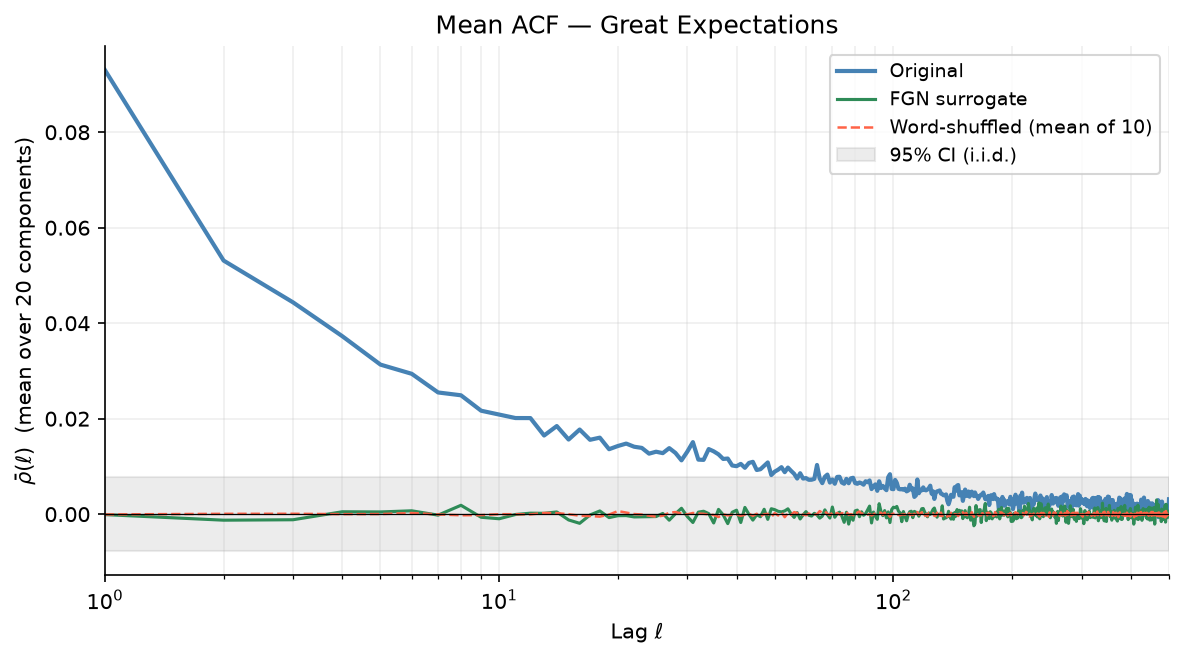
\includegraphics[width=0.72\textwidth]{figures/great_expectations_cut_clean/great_expectations_cut_clean_09_acf_mean_loglag.png}
  \caption{%
    \textbf{Mean ACF $\bar\rho(\ell)$ averaged over all $K=20$ PCA
    components --- \emph{Great Expectations} (Dickens).}
    Same colour conventions as the per-component ACF figure in the main text.
    The original text maintains positive mean autocorrelation well
    beyond the i.i.d.\ band across the full range of lags shown.
    The FGN surrogate and word-shuffled null are
    indistinguishable from the i.i.d.\ reference at all lags,
    confirming that rank-level long-range memory
    (present in the FGN by construction) does not propagate to the
    semantic projection space.
  }
  \label{fig:acf_mean}
\end{figure}




\begin{figure}[H]
  \centering
  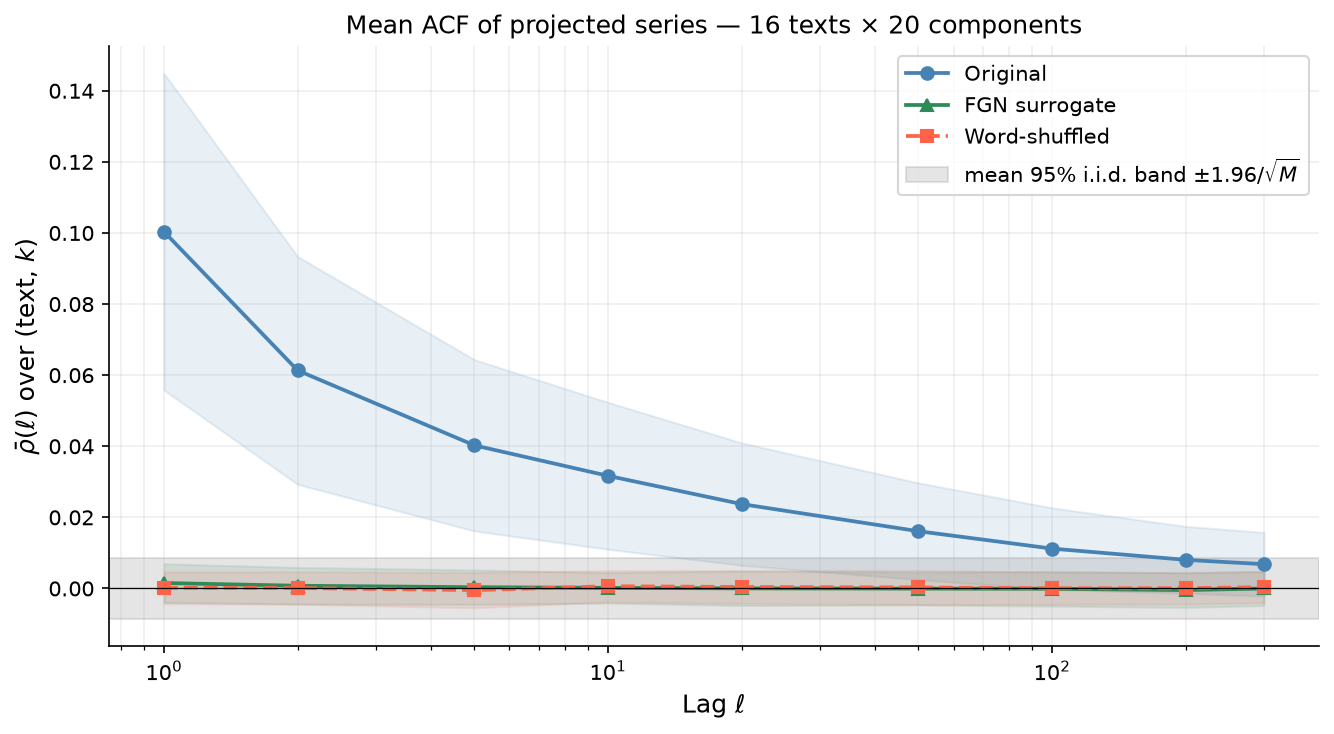
\includegraphics[width=\textwidth]{figures/acf_corpus_mean_decay.png}
  \caption{%
    \textbf{Mean ACF $\bar\rho(\ell)$ of projected series across the
    corpus of 16 texts and $K=20$ components, as a function of lag
    $\ell$ (log scale).}
    Shaded bands: $\pm 1$ standard deviation over
    $({\rm text}, k)$ pairs.
    Grey band: mean 95\% i.i.d.\ confidence band
    $\pm 1.96/\sqrt{M}$.
    Blue circles: original filtered text.
    Green triangles: FGN surrogate.
    Red squares: word-shuffled null.
    The original maintains significant positive ACF across all lags
    tested ($\ell = 1, \ldots, 300$).
    Both null models are indistinguishable from zero at all lags.
  }
  \label{fig:acf_corpus_decay}
\end{figure}


\begin{figure}[H]
  \centering
  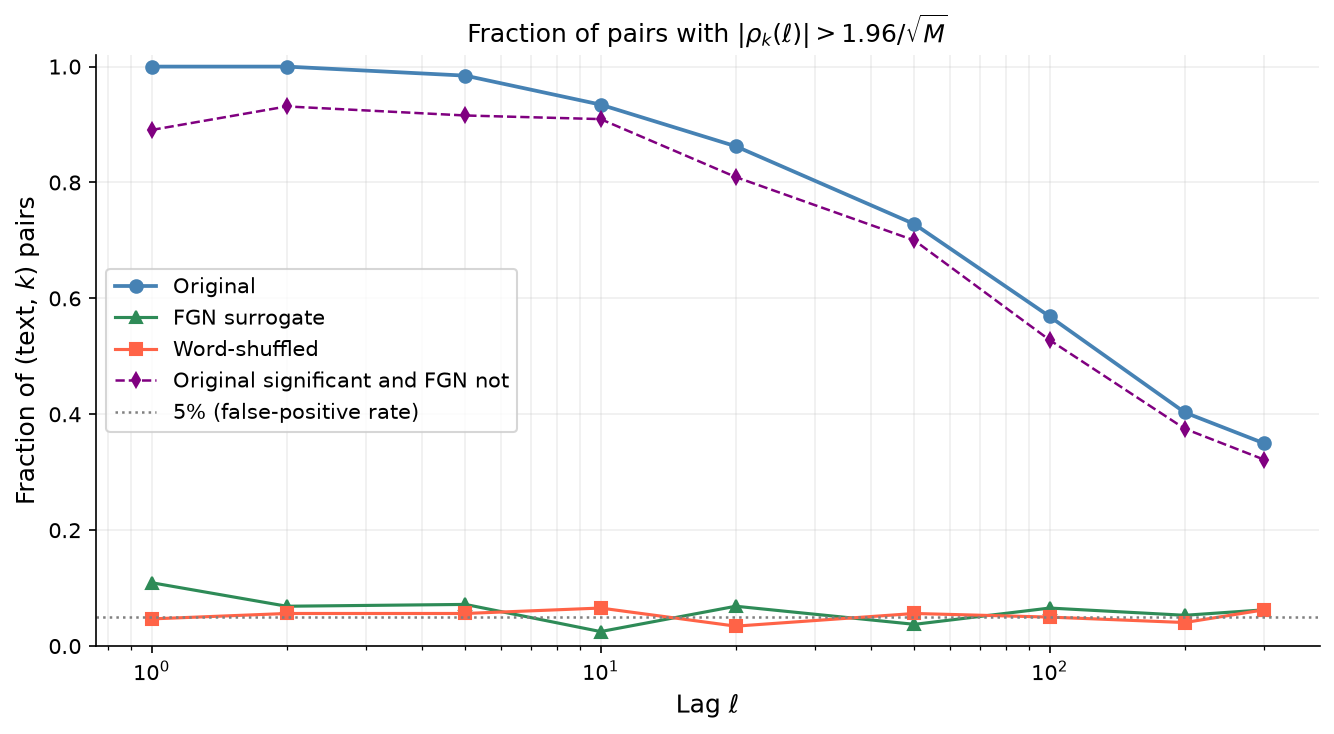
\includegraphics[width=0.72\textwidth]{figures/acf_corpus_frac_significant.png}
  \caption{Fraction of text--component pairs with significant ACF as
  a function of lag $\ell$ (log scale). Blue: original; green: FGN;
  red: word-shuffled; purple dashed: original significant and FGN not.
  The original remains clearly separated from both controls through
  lags of order $10^2$. The short-lag FGN excess is concentrated
  disproportionately in PC1, the component most affected by the
  embedding-geometry artefact discussed in the preprocessing section of the main text.}
  \label{fig:acf_corpus_frac}
\end{figure}



\begin{figure}[H]
  \centering
  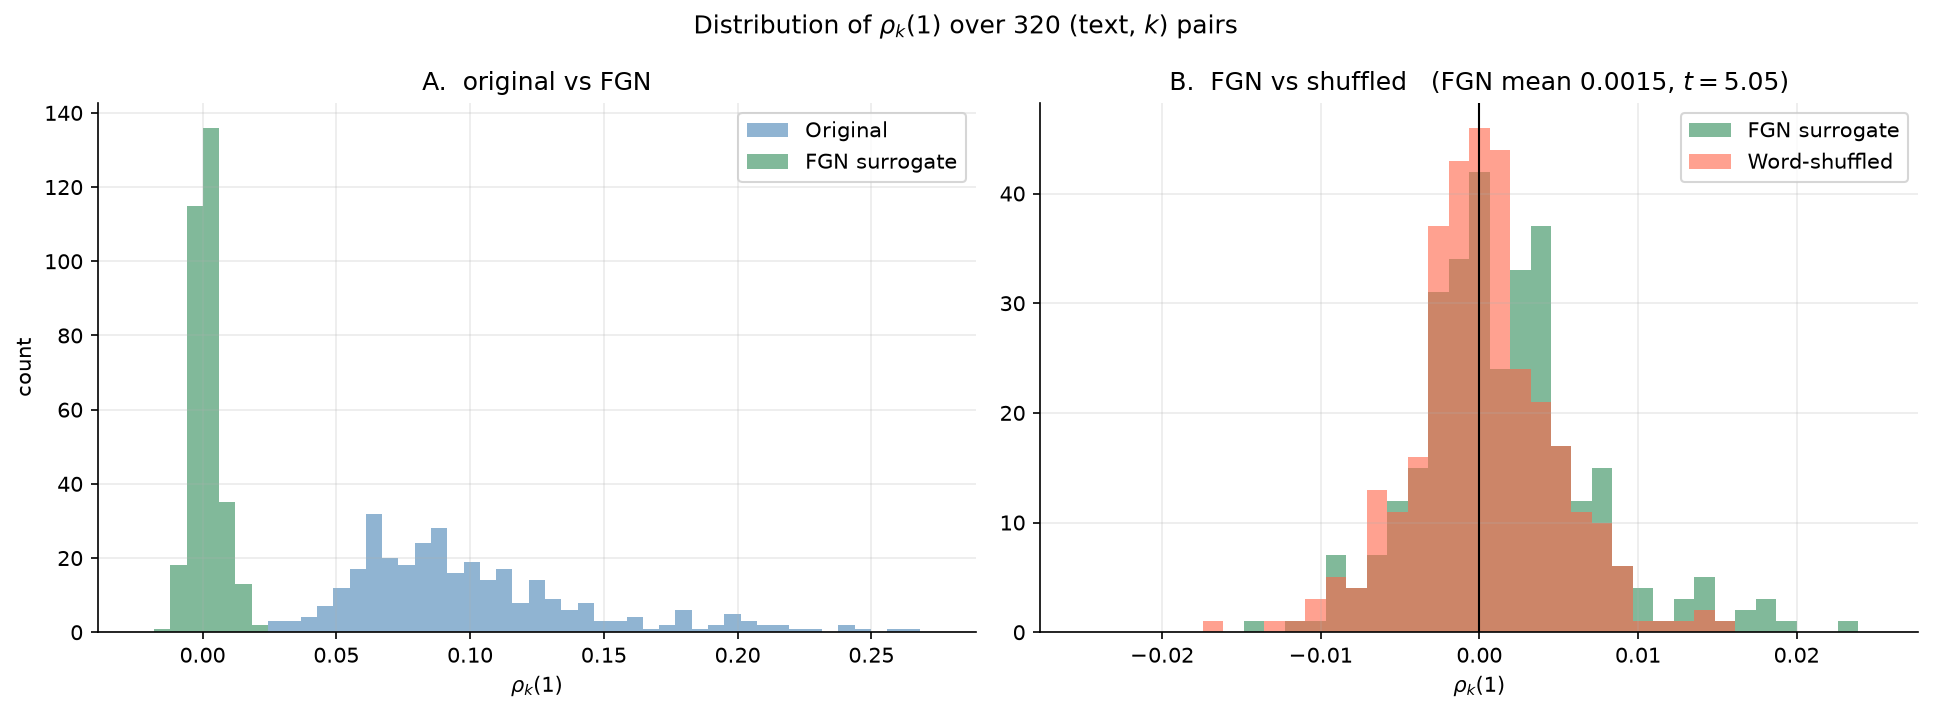
\includegraphics[width=\textwidth]{figures/acf_corpus_rho1_distribution.png}
  \caption{%
    \textbf{Distribution of $\rho_k(1)$ over $320$ (text, $k$) pairs.}
    \textbf{Panel A}: original (blue) and FGN (green).
    The two distributions are completely separated: every original pair
    exceeds its own text-specific i.i.d.\ band (which ranges from
    $0.004$ to $0.015$ across the corpus), while nearly all FGN pairs
    fall inside it.
    \textbf{Panel B}: FGN (green) and word-shuffled (red) on an
    expanded scale.
    Both are centred near zero; a $t$-test gives $t = 5.05$
    for $\bar\rho^{\rm FGN}(1) = 0$ but the effect size is
    negligible ($0.002$) relative to the orig--null gap ($0.098$).
  }
  \label{fig:acf_corpus_rho1}
\end{figure}
\clearpage
\section{Full numerical tables}
\begin{table}[H]
\centering
\caption{ACF of projections at lags $\ell = 1$ and $\ell = 100$ for
\emph{Great Expectations}. The i.i.d.\ reference band is
$\pm 1.96/\sqrt{M} = \pm 0.0077$. Values clearly outside the band are
in bold; values that round to the band edge are left unmarked.}
\label{tab:acf_summary}
\small
\begin{tabular}{r rr r rr}
\toprule
 & \multicolumn{2}{c}{$\rho_k(1)$} & \phantom{x}
 & \multicolumn{2}{c}{$\rho_k(100)$} \\
\cmidrule{2-3} \cmidrule{5-6}
$k$ & Orig & FGN && Orig & FGN \\
\midrule
 1 & \textbf{0.060} &    0.004 &&    0.008 &    0.004 \\
 2 & \textbf{0.208} &    0.007 && \textbf{0.015} &    0.004 \\
 3 & \textbf{0.136} & $-$0.002 && \textbf{0.018} &    0.004 \\
 4 & \textbf{0.123} & $-$0.003 &&    0.008 & $-$0.003 \\
 5 & \textbf{0.086} & $-$0.002 &&    0.004 & $-$0.004 \\
 6 & \textbf{0.121} &    0.004 &&    0.005 & $-$0.001 \\
 7 & \textbf{0.127} &    0.002 &&    0.007 & $-$0.003 \\
 8 & \textbf{0.103} &    0.001 &&    0.004 &    0.003 \\
 9 & \textbf{0.082} & $-$0.002 &&    0.008 &    0.001 \\
10 & \textbf{0.083} &    0.004 &&    0.003 &    0.003 \\
\midrule
 & \multicolumn{5}{l}{\emph{(k=11..20 all have $|\rho^{\rm FGN}(1)| \le 0.007$)}} \\
\bottomrule
\end{tabular}
\end{table}



\begin{table}[H]
\centering
\caption{DFA scaling exponents $\alpha_k$ of projected series
$x_t^{(k)}$ for \emph{Great Expectations} (Dickens, $\alpha=0.689$).
Every original value exceeds the shuffled reference by more than
$2\sigma$ (the spread over the ten shuffled realisations is
$\sigma\simeq0.004$), and every FGN value lies within $0.05$ of $0.5$.}
\label{tab:dfa_proj}
\scriptsize
\setlength{\tabcolsep}{4pt}
\begin{tabular}{r ccc r ccc}
\toprule
$k$ & $\alpha^{\rm orig}$ & $\alpha^{\rm FGN}$ &
    $\alpha^{\rm surr}$ &
$k$ & $\alpha^{\rm orig}$ & $\alpha^{\rm FGN}$ &
    $\alpha^{\rm surr}$ \\
\midrule
 1 & 0.605 & 0.511$\sim$ & 0.501 &
11 & 0.57 & 0.506$\sim$ & 0.500 \\
 2 & 0.681 & 0.500$\sim$ & 0.491 &
12 & 0.642 & 0.493$\sim$ & 0.502 \\
 3 & 0.693 & 0.518$\sim$ & 0.495 &
13 & 0.564 & 0.512$\sim$ & 0.500 \\
 4 & 0.634 & 0.514$\sim$ & 0.499 &
14 & 0.595 & 0.484$\sim$ & 0.497 \\
 5 & 0.64 & 0.486$\sim$ & 0.496 &
15 & 0.645 & 0.486$\sim$ & 0.497 \\
 6 & 0.633 & 0.515$\sim$ & 0.501 &
16 & 0.579 & 0.505$\sim$ & 0.494 \\
 7 & 0.647 & 0.504$\sim$ & 0.498 &
17 & 0.586 & 0.511$\sim$ & 0.493 \\
 8 & 0.633 & 0.469$\sim$ & 0.497 &
18 & 0.617 & 0.515$\sim$ & 0.507 \\
 9 & 0.643 & 0.482$\sim$ & 0.494 &
19 & 0.595 & 0.489$\sim$ & 0.505 \\
10 & 0.630 & 0.482$\sim$ & 0.503 &
20 & 0.622 & 0.495$\sim$ & 0.502 \\
\midrule
\multicolumn{4}{l}{\textbf{Mean}} &
\multicolumn{4}{l}{$\bar\alpha^{\rm orig}=0.623\pm0.034$ \quad
                   $\bar\alpha^{\rm FGN}=0.499\pm0.014$ \quad
                   $\bar\alpha^{\rm surr}=0.499\pm0.004$}\\
\bottomrule
\end{tabular}
\end{table}

\end{document}